% Capíulo 3
\chapter{Estudo de Análise da Compatibilidade a Múltiplas Versões da API Android}
\label{ch:estudo}

Este capítulo apresenta o estudo realizado para análise do suporte de aplicações
existentes à múltiplas versões da API da plataforma Android. Foram analisados o
códi- go-fonte de 41 aplicações únicas com o objetivo de identificar e caracterizar
as técnicas de implementação de variabilidades.

O restante do capítulo está organizado da seguinte maneira: 
a seção \ref{sec:objetivos} destaca os objetivos do estudo e as questões de pesquisa.
Proposições e hipóteses são formalizadas na seção \ref{sec:hipoteses}.
A seção \ref{sec:aplicacoes-alvo} apresenta os critérios de seleção das aplicações
alvo do estudo, bem como as aplicações selecionadas.
A seção \ref{sec:procedimentos} descreve os procedimentos adotados para responder
cada questão de pesquisa. 
A seção \ref{sec:resultados} apresenta os resultados do estudo, que são discutidos na
seção \ref{sec:discussao}.
Por fim, as ameaças à validade são reportadas na seção \ref{sec:ameacas}.

\section{Objetivos do Estudo e Questões de Pesquisa} \label{sec:objetivos}

Nosso estudo foi realizado com o objetivo de caracterizar, entender e analisar
como as aplicações Android lidam com múltiplas versões da API da plataforma, além
do impacto deste suporte no código-fonte das aplicações. Para atingir este objetivo,
o estudo foi guiado pelas seguintes questões de pesquisa (QPs):

\begin{itemize}
	\item \textbf{QP1}: Quais são as técnicas que aplicações atuais usam para manter
	compatibilidades com as diversas versões da API do Android? O objetivo dessa questão
	é indicar quais as técnicas vem sendo utilizadas e suas características, auxiliando
	desenvolvedores a decidirem o que e quando utilizar em suas aplicações.
	\item \textbf{QP2}: Qual o subconjunto de novas funcionalidades da plataforma que são
	mais utilizadas por aplicações compatíveis com versões antigas da API? Esse levantamento
	auxilia desenvolvedores de aplicações Android a identificar os elementos que eles, provavelmente,
	precisarão utilizar em suas aplicações, permitindo a concentração de esforços nesses componentes.
	\item \textbf{QP3}: Qual o esforço necessário para aumentar a compatibilidade da aplicação 
	com um maior número de APIs de versões anteriores da plataforma? Estabelecer uma versão
	elevada de API para execução do aplicativo pode significar deixar de atender um grande
	mercado potencial. Assim, a resposta para essa questão dará aos desenvolvedores um
	indicativo estimado do trabalho que terão para aumentar seu mercado potencial.
	\item \textbf{QP4}: Qual a incidência de código morto em função da versão da API do Android? 
	A evolução da API mínima exigida pelas aplicações, aqui no sentido de edição da configuração
	no arquivo de manifesto, associada à execução condicional pode resultar em código-morto.
	Analisamos as aplicações para determinar se isso tem ocorrido com frequência e em qual volume.
\end{itemize}

\section{Proposições e Hipóteses} \label{sec:hipoteses}

A partir das questões de pesquisas apresentadas anteriormente, algumas proposições
e hipóteses foram elaboradas para validação de que as respostas à tais questões podem
de fato serem úteis para academia e indústria de desenvolvimento de aplicações Android.
A estrutura de proposições e hipóteses baseia-se nas orientações do guia proposto por 
Runeson et al. \cite{Runeson2012} e seguem listadas abaixo.

\subsection{Relacionada à QP1}
	\begin{itemize}
		\item \textbf{Proposição P1}: Se a plataforma oferece suporte para múltiplas versões
		da API e tal suporte tem impacto no mercado em potencial então os desenvolvedores
		utilizam tal recurso.
		\item \textbf{Hipótese H1}: As aplicações utilizam pelo menos uma das técnicas disponíveis
		para oferecer suporte a múltiplas versões da API.
	\end{itemize}

\subsection{Relacionada à QP2}
	\begin{itemize}
		\item \textbf{Proposição P2}: Se a cada nova versão da plataforma são disponibilizados
		diversos novos recursos então deve existir um subconjunto que é mais utilizado no 
		contexto de suporte a múltiplas versões da API.
		\item \textbf{Hipótese H2}: Existe um subconjunto dos novos recursos da API que é
		mais utilizado no contexto de suporte a múltiplas versões da API.
	\end{itemize}

\subsection{Relacionada à QP3}
	\begin{itemize}
		\item \textbf{Proposição P3}: Se as aplicações utilizam apenas APIs mais recentes,
		não possuindo um histórico de uso de APIs antigas, então elas foram desenvolvidas
		sem a preocupação de oferecer suporte às versões antigas da API o que, possivelmente,
		a leva a perder uma fatia do mercado de aplicações.
		\item \textbf{Hipótese H3}: As aplicações podem aumentar o seu mercado potencial com
		baixo esforço em termos de desenvolvimento (alterações em seu código-fonte).
	\end{itemize}

\subsection{Relacionada à QP4}
	\begin{itemize}
		\item \textbf{Proposição P4}: Se as aplicações utilizam execução condicional para
		execução de determinados trechos de códigos e a sua API mínima exigida é superior
		à necessária para execução do trecho de código, então tal trecho de código é código-morto.   
		\item \textbf{Hipótese H4}: As aplicações possuem código-morto, que só seriam executados
		na presença de APIs antigas.
	\end{itemize}

\section{Aplicações Alvo do Estudo} \label{sec:aplicacoes-alvo}

As aplicações utilizados no estudo são aplicações \textit{open-source} populares,
com um mínimo de 6 mil linhas de código, contabilizados arquivos Java e XML, e de
categorias diversas. Uma das aplicações possui 10 mil \textit{downloads} na Google
Play, outra possui 50 mil \textit{downloads} e as demais mais de 100 mil.

A natureza das nossas questões de pesquisa exigiu a análise de grupos diferentes
de aplicações para determinadas questões, com critérios de seleção adicionais aos
citados anteriormente. Assim, definimos 3 grupos de aplicações, apresentados a seguir.

\subsection{Grupo 1 - Aplicações usando API da plataforma com grande variação de versões}
Aplicações do grupo 1 possuem uma diferença de pelo menos 7 versões entre a API mínima e
a API alvo. Tais aplicações foram utilizadas para responder às questões QP1 e QP2 e são
listadas na tabela
\ref{tab:grupo1}. São 25 aplicações nesse grupo.

\begin{table}[!htb] % TODO posicionar melhor essa tabela
  \centering
  \caption{Aplicações usando API da plataforma com grande variação de versões}
  \begin{tabular}{| l | l | r | r | r | r |}
  	\hline
  	% rótulo das columnas
  	\multicolumn{1}{|c|}{\textbf{Aplicação}} &
  	\multicolumn{1}{c|}{\textbf{Categoria}} &
 	\multicolumn{1}{c|}{\textbf{Downloads}} & 
 	\begin{tabular}[c]{@{}c@{}}
 		\textbf{API}\\ \textbf{Mínima}
 	\end{tabular} &
 	\begin{tabular}[c]{@{}c@{}}\textbf{API}\\ \textbf{Alvo}\end{tabular} &
 	\multicolumn{1}{c|}{\textbf{KLoc}} \\ \hline
 	%dados
 	Wififixer 		& Ferramentas 			& 1.000.000   &  7 & 23 &   9 \\ \hline
 	AnySoftKeyBoard & Ferramentas 			& 1.000.000   &  7 & 23 & 180 \\ \hline
 	Telegram 		& Comunicação 			& 100.000.000 &  9 & 23 & 169 \\ \hline
 	AntennaPod  	& Mídia e Video 		& 100.000 	  & 10 & 23 &  65 \\ \hline
 	Google I/O   	& Livros e Referências 	& 500.000 	  & 14 & 22 &  52 \\ \hline
 	Firefox    		& Comunicação 			& 100.000.000 & 15 & 22 & 233 \\ \hline
 	AnkiDroid     	& Educação 				& 1.000.000   & 10 & 22 &  89 \\ \hline
 	K-9 Mail      	& Comunicação 			& 5.000.000   & 15 & 22 & 117 \\ \hline
 	C:Geo       	& Entretenimento 		& 1.000.000   &  9 & 21 & 123 \\ \hline
 	Zmanim        	& Estilo de Vida 		& 10.000 	  & 10 & 22 &  25  \\ \hline
 	\begin{tabular}[l]{@{}l@{}}
 		Simon Tatham's \\ Puzzles
 	\end{tabular} 	& Quebra-cabeças 		& 100.000 	  &  7 & 23 &   8  \\ \hline
 	Vuze Remote     & Ferramentas			& 100.000	  &  7 & 23 &  20 \\ \hline
 	VLC for Android & 
 	\begin{tabular}[l]{@{}l@{}} Reproduzir e \\
 	 		 editar vídeos \end{tabular}    & 50.000.000  &  8 & 23 &  65 \\ \hline
 	\begin{tabular}[l]{@{}l@{}}
 	 	DuckDuckGo \\ Search \& Stories
 	\end{tabular}   & Livros e referências  & 1.000.000   &  8 & 23 &  23 \\ \hline
 	\begin{tabular}[l]{@{}l@{}}
 		Shattered Pixel \\ Dungeon
 	\end{tabular} 	& RPG 					& 500.000     &  8 & 23 &  58 \\ \hline
 	Persian Calendar& Produtividade			& 100.000 	  &  8 & 23 &  10 \\ \hline
 	Free Mobile Netstat& Ferramentas  		& 100.000 	  &  8 & 23 &   6 \\ \hline
 	MyExpenses    & Finanças 			& 100.000     &  8 & 23 &  80 \\ \hline
    \begin{tabular}[l]{@{}l@{}}
    	Simple Last.fm \\ Scrobbler
    \end{tabular} 	   & Música e áudio     & 500.000     &  7 & 22 &  10 \\ \hline
    Document Viewer	   & Produtividade		& 500.000 	  &  8 & 22 &  77 \\ \hline
	OpenTasks		   & Produtividade      & 100.000     &  8 & 22 &  23 \\ \hline
	\begin{tabular}[l]{@{}l@{}}
		Terminal Emulator \\ for Android
	\end{tabular} 	   & Ferramentas		& 10.000.000  &  4 & 22 &  18 \\ \hline
	ConnectBot		   & Comunicação	    & 1.000.000   &  4 & 22 &  24 \\ \hline
	Quick Dice Roller  & Ferramentas		& 100.000 	  &  4 & 21 &  35 \\ \hline
	\begin{tabular}[l]{@{}l@{}}
		BatteryBot Battery \\ Indicator
	\end{tabular} 	   & Ferramentas		& 5.000.000   &  7 & 22 &  6 \\ \hline
  \end{tabular}
  \label{tab:grupo1}
\end{table}

\subsection{Grupo 2 - Aplicações usando apenas APIs mais recentes}
Aplicações do grupo 2 possuem um alto valor de API mínima mas não tem um histórico de suporte
às versões anteriores. Para esse estudo, as versões iguais ou superiores à 16 foram consideradas
como alta. Versões inferiores a esta representam 3.4\% do mercado mundial, conforme pode ser visto
na figura \ref{fig:platform_versions}. E para caracterizar ausência de um histórico de suporte
às versões anteriores,
consideramos aquelas cuja API mínima inicial seja igual ou superior a 11. Tais aplicações foram
utilizadas para responder à questão QP3 e estão listadas na tabela \ref{tab:grupo2}. São 10
aplicações nesse grupo.

\begin{table}[!htbp]
  \small	
  \centering
  \caption{Aplicações usando apenas APIs mais recentes}
  \begin{tabular}{| l | l | r | r | r | r |}
  	\hline
  	% rótulo das columnas
  	\multicolumn{1}{|c|}{\textbf{Aplicação}} &
  	\multicolumn{1}{c|}{\textbf{Categoria}} &
 	\multicolumn{1}{c|}{\textbf{Downloads}} & 
 	\begin{tabular}[c]{@{}c@{}}
 		\textbf{API}\\ \textbf{Mínima} \\ \textbf{Inicial}
 	\end{tabular} &
 	\begin{tabular}[c]{@{}c@{}}\textbf{API}\\ \textbf{Mínima}\\ \textbf{Atual}\end{tabular} &
 	\multicolumn{1}{c|}{\textbf{KLoc}} \\ \hline
 	% dados
 	AcDisplay 		& Personalização 		& 1.000.000   & 19 & 16 & 40 \\ \hline
 	Dash Clock		& Personalização		& 1.000.000   & 17 & 17 & 15 \\ \hline
 	Focal (Beta) 	& Fotografia 			& 500.000	  & 16 & 16 &  16 \\ \hline
 	\begin{tabular}[l]{@{}l@{}}
 	 		Hangar - Smart \\ app shortcuts
 	\end{tabular}	& Ferramentas 		& 50.000 	  & 16 & 16 &  12 \\ \hline
 	Indic Keyboard  & Ferramentas 	& 100.000 	  & 14 & 16 &  81 \\ \hline
 	\begin{tabular}[l]{@{}l@{}}
 	 	 	Numix Circle \\ icon pack
 	\end{tabular}   & Personalização    	& 100.000 	  & 11 & 16 &   8 \\ \hline
 	SnoopSnitch     & Ferramentas 			& 100.000     & 14 & 16 &  17 \\ \hline
 	Termux      	& Ferramentas 			& 100.000	  & 21 & 21 &  10 \\ \hline
 	\begin{tabular}[l]{@{}l@{}}
 	 		WiFiAnalyzer \\ (open-source)
 	\end{tabular}   & Ferramentas 			& 100.000     & 22 & 21 &  12 \\ \hline
 	\begin{tabular}[l]{@{}l@{}}
 		Yaac - \\ IRC Client
 	\end{tabular} 	& Ferramentas 			& 50.000 	  & 16 & 16 &  12  \\ \hline
 	\end{tabular}
  \label{tab:grupo2}
\end{table}


\subsection{Grupo 3 - Aplicações usando APIs recentes com histórico de uso de APIs antigas}
Aplicações do grupo 3 possuem um alto valor de API mínima e também um histórico
de suporte às versões anteriores. Para esse grupo de aplicações, consideramos
aquelas cuja versão da API seja igual ou superior a 15 e a API mínima inicia
menor ou igual a 8. Tais aplicações foram utilizadas para responder à questão QP4 e
estão listadas na tabela \ref{tab:grupo3}.
São 7 aplicações nesse grupo.

\begin{table}[!htbp]
  \small
  \centering
  \caption{Aplicações usando APIs recentes com histórico de uso de APIs antigas}
  \begin{tabular}{| l | l | r | r | r | r |}
  	\hline
  	% rótulo das columnas
  	\multicolumn{1}{|c|}{\textbf{Aplicação}} &
  	\multicolumn{1}{c|}{\textbf{Categoria}} &
 	\multicolumn{1}{c|}{\textbf{Downloads}} & 
 	\begin{tabular}[c]{@{}c@{}}
 		\textbf{API}\\ \textbf{Mínima} \\ \textbf{Inicial}
 	\end{tabular} &
 	\begin{tabular}[c]{@{}c@{}}\textbf{API}\\ \textbf{Mínima}\\ \textbf{Atual}\end{tabular} &
 	\multicolumn{1}{c|}{\textbf{KLoc}} \\ \hline
 	% dados
 	AFWall+ 		& Ferramentas	 		& 500.000     & 7  & 15 & 32 \\ \hline
 	aMetro			& 
 	\begin{tabular}[l]{@{}l@{}}
 	 	Mapas e \\ Navegação \end{tabular}	& 100.000	  & 3 & 15 &  10 \\ \hline
 	K-9 Mail  		& Comunicação 		& 5.000.000	  &  3 & 15 &  117 \\ \hline
 	\begin{tabular}[l]{@{}l@{}}
 	 	 	Orbot Proxy \\ com Tor
 	\end{tabular}   & Comunicação    	& 5.000.000 	  & 4 & 16 & 33 \\ \hline
 	Ringdroid     	&
 	\begin{tabular}[l]{@{}l@{}} Reproduzir e \\
 	 	 	Editar Vídeos \end{tabular}	& 50.000.000	  & 4 & 16 &   6 \\ \hline
 	Transdrone      & Ferramentas 		& 100.000	      & 4 & 15 &  36 \\ \hline
 	\begin{tabular}[l]{@{}l@{}}
 	 		Vanilla Music
 	\end{tabular}   & Música e Áudio 			& 500.000     &  3 & 15 & 25 \\ \hline
 	\end{tabular}
  \label{tab:grupo3}
\end{table}

\section{Procedimentos} \label{sec:procedimentos}

Uma vez selecionadas as aplicações alvos do estudo, foi realizada a atividade de
análise das aplicações para buscar respostas às questões de pesquisa. A seguir,
descrevemos os procedimentos adotados. 

\subsection{Questões QP1 e QP2}
Para responder às questões de pesquisa QP1 e QP2, os procedimentos adotados foram os
seguintes:

\begin{enumerate}
	\item Remoção das anotações \texttt{@TargetAPI}, \texttt{@SuppressWarnings},
	 	\texttt{@SuppressLint} do código-fonte da aplicação. Essas remoções foram
	 	 necessárias porque tais anotações servem para silenciar o Lint, omitindo 
	 	 ocorrências do relatório; 
	\item Execução do Android Lint na aplicação;
	\item Para cada ocorrência de NewApi, o contexto era analisado de forma manual
		para determinar se:
		\begin{itemize}
			\item Trata-se da implementação do padrão Execução Condicional
				\cite{Santos2012};
			\item Implementação é baseada em padrões de projeto \cite{Gamma}; 
			\item Ou algum outro mecanismo que evitasse a chamada em uma versão
			da API cujo recurso está ausente;
		\end{itemize}
	\item Para cada ocorrência de NewApi, de forma semiautomática, o elemento da API
		era classificado de acordo com a taxonomia apresentada na seção \ref{sec:taxonomia};
	\item Nos aplicativos que utilizam pacote de compatibilidade, os elementos foram
		 classificados na taxonomia com uma busca pelos \texttt{import}'s  presentes
		 nas classes das aplicações.
\end{enumerate}

\subsection{Questão QP3}
Para responder à questão de pesquisa QP3, os procedimentos adotados foram os
seguintes:

\begin{enumerate}
	\item Remoção das anotações \texttt{@TargetAPI}, \texttt{@SuppressWarnings},
		 	\texttt{@SuppressLint} do código-fonte da aplicação;
	\item Execução do Android Lint na aplicação;
		\begin{itemize}
			\item Esse resultado era salvo para uso futuro;
		\end{itemize}
	\item Edição da API mínima da aplicação para a versão imediatamente inferior à atual
		e presente na tabela \ref{fig:platform_versions};
		\begin{itemize}
			\item APIs ausentes dessa tabela foram descartadas por não representarem
			um mercado minimamente significativo;
		\end{itemize}
	\item Nova execução do Android Lint na aplicação;
		\begin{itemize}
			\item Esse resultado era comparado com o obtido em 2;
			\item Se a quantidade de NewApi fosse a mesma, voltávamos para 3, se não
			o resultado é analisado em maiores detalhes, como a taxonomia, a dependência
			do recurso pela aplicação e como a ocorrência poderia ser tratada.
		\end{itemize}
\end{enumerate}

\subsection{Questão QP4}
Para responder à questão de pesquisa QP4 os procedimentos adotados foram os seguintes:

\begin{enumerate}
	\item Pesquisa textual por \texttt{VERSION.SDK\_INT} em todos os arquivos da
		aplicação;
	\item Quando \texttt{VERSION.SDK\_INT} fazia parte de um execução condicional, ou equivalente, relacionada a uma versão da API inferior a API mínima da aplicação, o código da aplicação era refatorado de forma a remover todo o código-morto.
	\item Contabilização e sumarização das linhas de código e arquivos removidos.
\end{enumerate}

\section{Resultados do Estudo} \label{sec:resultados}

Essa seção apresenta os resultados do estudo. As subseções estão organizadas em termos
das questões de pesquisa (Seção \ref{sec:objetivos}).

\subsection{Quais são as técnicas que aplicações atuais usam para manter
compatibilidades com as diversas versões da API do Android?} \label{subsec:tecnicas_usadas}

Para permitir o uso de novos recursos da API em aplicações que ainda desejam
oferecer suporte a dispositivos com vers da API mais antigas, foram
identificadas 3 estratégias de implementação: (i) pacote de compatibilidade;
(ii) re-implementação de recurso da API e (iii) uso explícito da nova API.
Tais mecanismos podem ser utilizados em conjunto.

A figura \ref{fig:forma_suporte} apresenta a quantidade total de aplicações de
cada estratégia. Pacote de compatibilidade foi utilizada por 23 aplicações,
re-implementação de recurso por 14, e uso explícito da nova API por 22.

\begin{figure}[!htbp]
	\centering 
  	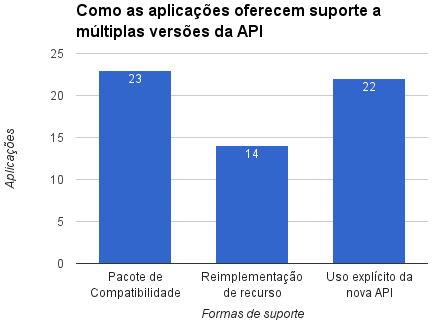
\includegraphics[scale=0.75]{imagens/forma_suporte}
  	\textsf{\caption{Como as aplicações oferecem suporte a múltiplas versões da API}
  	        \label{fig:forma_suporte}}
\end{figure}

A técnica de uso explícito da nova API pode causar um erro na aplicação caso seja
executado em um dispositivo com versão da API inferior àquela em que o componente
utilizado foi adicionado. Assim, é necessário algum mecanismo para evitar que isso
aconteça. O mecanismo primário padrão é um comando condicional. No entanto, existem
diversas maneiras de implementação de tal comando condicional, desde uma instrução
\texttt{if} logo acima da linha de código, até a utilização de padrões de projeto,
em que o \texttt{if} determina a criação de objetos baseado na versão da API Android
do dispositivo, por exemplo.

O gráfico apresentado na figura \ref{fig:alternativas_EC} mostra as diferentes
alternativas de projeto encontradas nas aplicações analisadas para implementação
de execução condicional em torno das linhas com ocorrências de Lint NewApi. Tais
resultados foram obtidos a partir da análise do resultado da execução do Lint NewApi
nas aplicações. Execução condicional \cite{Santos2012} indireta e uso de padrões
de projeto foram as técnicas mais comum, estando presente em 16 aplicações analisadas.
Execução condicional direta e suporte implícito foram utilizadas em 12 aplicações cada.
6 aplicações deixaram de fazer o tratamento de algumas ocorrências, 5 aplicações possuem ocorrências dentro de métodos que nunca serão executados e, por fim, uma aplicação
utilizou tratamento de exceção para evitar erro durante a execução.

\begin{figure}[htb]
	\centering 
  	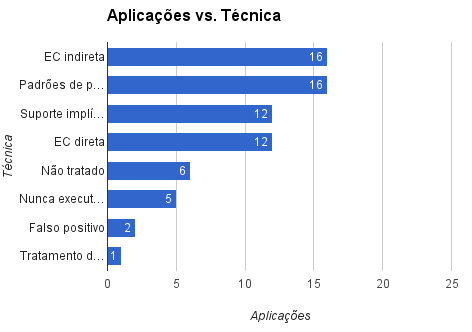
\includegraphics[scale=0.75]{imagens/alternativas_EC}
  	\textsf{\caption{Quantidade de aplicações que utilizaram cada técnica para
  						tratamento de ocorrência de NewApi}
  	        \label{fig:alternativas_EC}}
\end{figure}

Também foram detectadas ocorrências de falsos positivos em duas aplicações.
Falso positivo acontece quando um determinado método \texttt{X()} qualquer foi
adicionado em uma classe da API em versão superior da aplicação, posteriormente
uma classe estende essa classe da API e implementa o método \texttt{X()}, mas
o Lint NewApi não identifica essa implementação, reportando o falso problema.

A figura \ref{fig:falso_positivo} exemplifica tal situação com um dos casos reais 
encontrados. O método \texttt{invalidadeOptionsMenu()} foi adicionado à classe
\texttt{Activity} na versão 11 da API, portanto ele não pode ser chamado em
versões anteriores. Assim, foi disponibilizado através da re-implementação na classe 
\texttt{AppCompatActivity} do pacote de compatibilidade e que herda de \texttt{Activity}.
Na aplicação Telegram, cuja API mínima é 10, existe uma classe que estende de 
\texttt{AppCompatActivity}, \texttt{CastEnableActivity}, que é então estendida por 
\texttt{MediaPlayerActivity}. No método \texttt{onOptionsItemSelected()} é feita 
uma chamada para \texttt{invalidadeOptionsMenu()}. Tal chamada é indevidamente
indicada pelo Lint.

\begin{figure}[htb]
	\centering 
  	\includegraphics[scale=0.6]{imagens/falso_positivo}
  	\textsf{\caption{Diagrama de classe exemplificando situação de falso positivo do Lint}
  	        \label{fig:falso_positivo}}
\end{figure}

A figura \ref{fig:percentuais_forma_tratamento} apresenta os percentuais das
formas de tratamento para as ocorrências de NewApi. Foram analisadas um total
de 1556 ocorrências de NewApi. Desse total, 40,6\% foi tratado com EC indireta,
22,8\% com algum padrão de projeto, 18,9\% através de EC direta, 10,7\% utilizando
suporte implícito da plataforma, 5,3\% das ocorrências não foram devidamente tratadas.
Continuando a análise, 1,2\% das ocorrências estão dentro de métodos
que nunca serão executados e, por fim, duas pequenas frações de 0,3\% das ocorrências
foi utilizada tratamento de exceção ou são falsos positivos. Essas ocorrências de NewApi 
estão distribuídas em 22 aplicações (3 aplicações não apresentaram ocorrências de alguma 
NewApi).

\begin{figure}[htb]
	\centering 
  	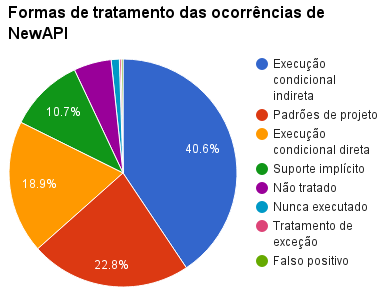
\includegraphics[scale=0.75]{imagens/percentuais_forma_tratamento}
  	\textsf{\caption{Percentuais de formas de tratamento das ocorrências de NewApi}
  	        \label{fig:percentuais_forma_tratamento}}
\end{figure}

O figura \ref{fig:padroes_por_aplicacao} apresenta os padrões de projeto utilizados
por quantidade de aplicações. O padrão \textit{Strategy} é o que mais foi utilizado
em um total de 12 aplicações. \textit{Template Method} e \textit{Null Object} foram 
utilizados por uma aplicação cada um. \textit{Proxy} foi utilizado por duas aplicações
Apenas uma aplicação utilizou dois padrões de projetos simultaneamente, \textit{Strategy}
e \textit{Proxy}. 

\begin{figure}[htb]
	\centering 
  	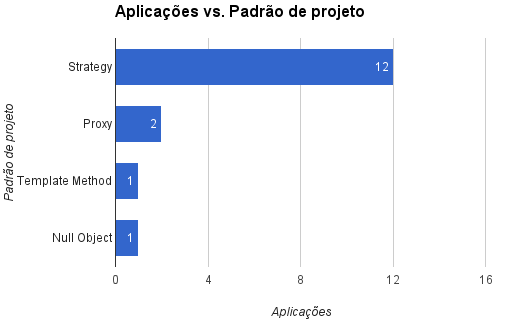
\includegraphics[scale=0.75]{imagens/padroes_por_aplicacao}
  	\textsf{\caption{Quantidade de aplicações que utilizaram padrões de projeto para
  						tratar ocorrências de NewApi}
  	        \label{fig:padroes_por_aplicacao}}
\end{figure}

O figura \ref{fig:percentuais_por_padrao} apresenta os percentuais dos padrões de
projeto utilizados como forma de tratamento para as ocorrências de NewApi. Do total
de 1554 ocorrências de NewApi analisadas, 355 (22,8\%) foram tratadas com algum
padrão de projeto. Sendo o mais comum o padrão \textit{Strategy}, responsável por
77,7\% (276) desse total. Os padrões \textit{Proxy} e \textit{Template Method}
foram responsáveis por 19,4\% e 2,3\% dos casos, respectivamente. \textit{Null Object}
foi utilizado por uma aplicação para tratar 2 (0,6\%) ocorrências.

\begin{figure}[htb]
	\centering 
  	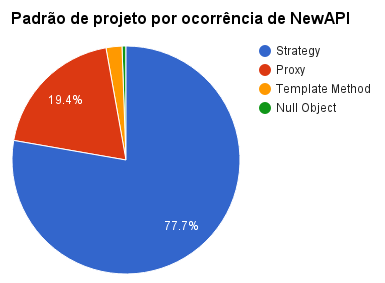
\includegraphics[scale=0.75]{imagens/percentuais_por_padrao}
  	\textsf{\caption{Percentuais de uso de padrões de projeto por ocorrências de NewApi}
  	        \label{fig:percentuais_por_padrao}}
\end{figure}

\subsection{Qual o subconjunto de novas funcionalidades da plataforma que são
mais utilizados por aplicações compatíveis com versões antigas da API?} \label{subsec:subjunto_api}

Analisamos as chamadas às novas APIs para determinar o subconjunto das
novas funcionalidades que são utilizadas pelas aplicações com suporte à versões
antigas da API. Os resultados foram contabilizados em função da taxonomia da API.
E, então, para as taxonomias mais comuns, apresentamos as classes mais recorrentes. 

\subsubsection{Pacote de Compatibilidade}

Para computar os dados relativos à pacote de compatibilidade, realizamos uma análise
estática sobre os projetos, identificando nos trechos de importação das classes Java
os elementos advindos do pacote \texttt{android.support}, excetuando os subpacotes
\texttt{annotations} e \texttt{tests}, pois estes além de não influenciarem na execução
da aplicação, não são analisadas pelo Lint NewApi. Os resultados foram contabilizados
em função da taxonomia da API. E então, para as taxonomias mais comuns, apresentamos
as classes mais recorrentes.

A tabela \ref{tab:elementos_pacote} apresenta os valores obtidos. Para cada taxonomia,
temos o número de aplicações que fizeram \texttt{import}’s do pacote de compatibilidade,
o total de \texttt{import}’s feitos, as importações únicas e a média de \texttt{import}’s 
por aplicação. Importações únicas significa que se uma classe é importada mais de uma vez, 
independente de aplicação, ela é contabilizado apenas uma vez. Em destaque os maiores 
valores de cada coluna, além das duas taxonomias mais significativas, que possuem uma
 maior média de \texttt{import}’s por aplicação.

\begin{table}[!htbp] % TODO posicionar melhor essa tabela
  \centering
  \caption{Elementos mais utilizados do pacote de compatibilidade}
  \begin{tabular}{| l | r | r | r | r |}
  	\hline
  	% rótulo das columnas
  	\multicolumn{1}{|c|}{\textbf{Taxonomia}} &
  	\multicolumn{1}{c|}{\textbf{Aplicações (A)}} &
 	\begin{tabular}[c]{@{}c@{}}
 		\textbf{Total de}\\ \textbf{import's (B)}
 	\end{tabular} &
 	\begin{tabular}[c]{@{}c@{}}\textbf{Importações}\\ \textbf{unicas}\end{tabular} &
 	\begin{tabular}[c]{@{}c@{}}\textbf{Média por}\\ \textbf{app (A/B)}\end{tabular} \\ \hline
 	%dados
 	animation 		& 1 			& 5   			&   4 			& 5  \\ \hline
 	\textbf{app}	& \textbf{22} 	& \textbf{849}  &  49 			& \textbf{39}\\ \hline
 	content 		& 17 			& 236 			&  11 			& 14  \\ \hline
 	graphics  		& 4 			& 9 			&   5 			& 2  \\ \hline
 	hardware   		& 1 			& 2 			&   1 			& 2  \\ \hline
 	media    		& 3 			& 15 			&   7 			& 5  \\ \hline
 	net     		& 1 			& 3   			&   1 			& 3  \\ \hline
 	os      		& 3 			& 6   			&   4 			& 2  \\ \hline
 	preference  	& 5 			& 99   			&  17 			& 20  \\ \hline
 	provider    	& 1 			& 12 			&   1			& 12   \\ \hline
 	text        	& 1 			& 1 			&   1 			& 1   \\ \hline
 	util       	 	& 9 			& 46 			&   9 			& 5   \\ \hline
 	view        	& 18 			& 233 			&  37 			& 13   \\ \hline
 	\textbf{widget} & 18			& 410 			&  \textbf{65} 	& 23   \\ \hline
  \end{tabular}
  \label{tab:elementos_pacote}
\end{table}

As taxonomias \textit{app} e \textit{widget} são as mais comuns. A primeira contém
classes de alto nível que encapsulam o modelo geral de aplicações Android. A última
fornece elementos de interface com o usuário para serem utilizados na tela da aplicação.
A figura \ref{fig:bloxplot_pacote_compatibilidade} apresenta diagramas de boxplot para as
distribuições de importações nas aplicações para essas duas taxonomias.

 \begin{figure}[htb]
 	\centering 
   	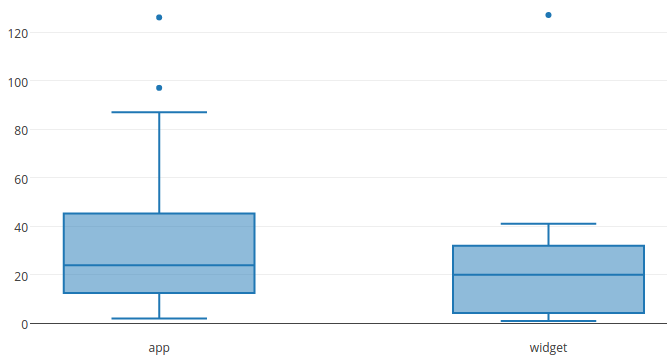
\includegraphics[scale=0.7]{imagens/bloxplot_pacote_compatibilidade}
   	\textsf{\caption{Distribuição de importações para as taxonomias \textit{app} e \textit{widget}}
   	        \label{fig:bloxplot_pacote_compatibilidade}}
 \end{figure}

\textit{App} possui o maior número importações, 849, e também maior média por aplicação,
39, distribuídos em 22 das 25 aplicações analisadas. Já \textit{widget} possui um número
bem menor
de importações, 410, embora bem mais alto que a terceira posição. Estando distribuídos em
18 aplicações. Além de possuir o maior número de chamadas únicas, 65. Isso demonstra que
os elementos de \textit{app} são mais restritos, enquanto \textit{widget} há uma
granularidade maior, havendo um maior acoplamento da aplicação a esses elementos em
relação aos elementos de \textit{app}.

Da taxonomia \textit{app}, a classe mais comum é \texttt{Fragment}, conforme apresenta
a tabela \ref{tab:elementos_app}. Além disso, outras três classes diretamente relacionadas
a fragmentos estão entre as 10 mais utilizadas: \texttt{DialogFragment}, 
\texttt{FragmentManager} e \texttt{FragmentActivity}.

\begin{table}[!htbp] % TODO posicionar melhor essa tabela
  \centering
  \caption{10 classes da taxonomia \textit{app} mais importadas do pacote de compatibilidade}
  \begin{tabular}{| l | r | r | r | }
  	\hline
  	% rótulo das columnas
  	\multicolumn{1}{|c|}{\textbf{Classes}} &
  	\multicolumn{1}{c|}{\textbf{Aplicações (A)}} &
 	\begin{tabular}[c]{@{}c@{}}
 		\textbf{Total de}\\ \textbf{importações (B)}
 	\end{tabular} &
 	\begin{tabular}[c]{@{}c@{}}\textbf{Média por}\\ \textbf{app (B/A)}\end{tabular} \\ \hline
 	%dados
 	v4.app.Fragment 			& 15 			& 144   		&   10 			  \\ \hline
 	v4.app.NotificationCompat	& 16 			& 80 			&   5 			  \\ \hline
 	v4.app.DialogFragment  		& 12 			& 76   			&   6 			  \\ \hline
 	v7.app.AlertDialog     		& 11 			& 72   			&   7			  \\ \hline
 	v7.app.AppCompatActivity  	& 14 			& 67   			&  5 			  \\ \hline
 	v4.app.FragmentManager    	& 16 			& 65 			&   4			   \\ \hline
 	v4.app.FragmentActivity    	& 12 			& 58 			&   5 			   \\ \hline
 	v4.app.LoaderManager       	& 7 			& 50 			&   5 			   \\ \hline
 	v7.app.ActionBar        	& 13 			& 37 			&  3 			   \\ \hline
 	v4.app.ActivityCompat 		& 14			& 25 			&  2 	   \\ \hline
  \end{tabular}
  \label{tab:elementos_app}
\end{table}

Se na taxonomia \textit{app} as importações tendem a elementos relacionados a
fragmentos, na taxonomia \textit{widget} houve uma maior dispersão. As classes
mais comuns são \texttt{RecyclerView} e \textit{Toolbar}. A primeira teve o
maior número de importações no total, enquanto a segunda, além de ter o segundo
maior valor de importações, é a que está presente em mais aplicações, 12 contra
9 para \textit{RecyclerView}. Os demais elementos aparecem em no máximo 9 aplicações,
com não mais que 26 importações no total. A tabela \ref{tab:elementos_widget}
apresenta as 10 classes da taxonomia \textit{widget} mais utilizadas.

\begin{table}[!htbp] % TODO posicionar melhor essa tabela
  \centering
  \caption{10 classes da taxonomia \textit{widget} mais importadas do pacote de compatibilidade}
  \begin{tabular}{| l | r | r | r | }
  	\hline
  	% rótulo das columnas
  	\multicolumn{1}{|c|}{\textbf{Classes}} &
  	\begin{tabular}[c]{@{}c@{}}
  	 		\textbf{Aplicações}\\ \textbf{(A)}
  	 	\end{tabular} &
 	\begin{tabular}[c]{@{}c@{}}
 		\textbf{Total de}\\ \textbf{importações (B)}
 	\end{tabular} &
 	\begin{tabular}[c]{@{}c@{}}\textbf{Média por}\\ \textbf{app (B/A)}\end{tabular} \\ \hline
 	%dados
 	v7.widget.RecyclerView 				& 9 	& 81 	  		&   9 			  \\ \hline
 	v7.widget.Toolbar					& 12 	& 52 			&   4 			  \\ \hline
 	v7.widget.LinearLayoutManager		& 9 	& 26   			&   3 			  \\ \hline
 	design.widget.Snackbar     			& 6 	& 23   			&   4			  \\ \hline
 	v7.widget.SearchView  				& 8		& 21   			&   3 			  \\ \hline
 	v4.widget.DrawerLayout    			& 9 	& 15 			&   2			   \\ \hline
 	design.widget.FloatingActionButton  & 4		& 13 			&   3 			   \\ \hline
 	v7.widget.PopupMenu       			& 5 	& 12 			&   2 			   \\ \hline
 	design.widget.TabLayout        		& 6		& 10 			&   3 			   \\ \hline
 	v4.widget.SwipeRefreshLayout 		& 5		& 10 			&   2 	   \\ \hline
  \end{tabular}
  \label{tab:elementos_widget}
\end{table}


\subsubsection{Re-implementação de Recursos}

Re-implementação de um recurso existente na API padrão pode ser uma re-imple- mentação
completamente própria, quando não existe cópia de código de outros projetos, ou pode
ser através da cópia do código-fonte do recurso na API padrão. Para este trabalho,
consideramos apenas a re-implementação através de cópia do código-fonte da API padrão.
O código-fonte do projeto Android é distribuído, preferencialmente, sob a licença Apache 
Software License, Versão 2.0 ("Apache 2.0") \cite{License}, e os direitos autorais
pertencem a \textit{Android Open Source Project}. Para indicar isso, todos os arquivos
do projeto possuem o seguinte preâmbulo:
\texttt{
\newline
/* \newline
 * Copyright (C) <YEAR> The Android Open Source Project \newline
 * \newline
 * Licensed under the Apache License, Version 2.0 (the "License"); \newline
 * you may not use this file except in compliance with the License. \newline
 * You may obtain a copy of the License at \newline
 * \\
 *      http://www.apache.org/licenses/LICENSE-2.0 \\
 * \\
 * Unless required by applicable law or agreed to in writing, software \\
 * distributed under the License is distributed on an "AS IS" BASIS, \\
 * WITHOUT WARRANTIES OR CONDITIONS OF ANY KIND, either express or implied. \\
 * See the License for the specific language governing permissions and \\
 * limitations under the License. \\
 */
} 

Assim, para verificarmos se as aplicações re-implementaram algum recurso através
da cópia de código da API padrão, realizamos uma busca textual nos arquivos Java
das aplicações por "Android Open Source Project". Para cada ocorrência, foi feita
uma pesquisa na documentação da API pelo nome da classe. Se não fosse encontrado
algo, era feita uma busca no Google, pela string "android <nome da classe>".
Analisamos as ocorrências  para determinar se o código havia sido copiado realmente
da API, de aplicações nativas do Android ou de projeto de exemplos oficiais,
desenvolvidas pela mesma equipe da plataforma. Em algumas situações, os códigos
tinham como origem o projeto Android, mas não faziam parte da API. Um exemplo disso
é a classe \texttt{NetworkActivity} que, embora desenvolvida pelo projeto Android e
possuir o preâmbulo citado acima, não faz parte da API. Ela é apresentada na
documentação \cite{NetworkUsage} e o código-fonte está no subdiretório \texttt{samples}
do repositório \cite{NetworkActivity}. Ocorrências como essa eram então descartadas.
Embora um número considerável de aplicações (14 de 25) tenha utilizado tal técnica,
foram usos bem pontuais e localizadas.

O conjunto de classes mais significativo diz respeito à implementação do pacote 
\texttt{android.animation} da API e ocorreu em 3 aplicações. O código presente
nas aplicações é proveniente da biblioteca NineOldAndroids\footnote{http://nineoldandroids.com/},
que disponibiliza seus arquivos para
download através do código-fonte e não em arquivos JAR ou algum outro mecanismo
para adição de dependência aos projetos, mas que isole o código da dependência
do código principal do projeto. Por esse motivo, tal código foi considerado
nessa análise. As classe \texttt{PreferenceFragment} e \texttt{PreferenceManager}
foram também re-implementadas por 3 aplicações.

A classe \texttt{android.util.Base64}, utilizada para codificação e decodificação
da representação de dados binários em Base64 \cite{RFC4648}, foi a classe mais
recorrente, detectada em 5 aplicações. Outras mais de 30 classes com propósitos 
diversos também foram re-implementadas, no entanto, em não mais de uma aplicação.

\subsubsection{Uso explícito da nova API}

Para determinar o subconjunto das novas funcionalidades da API que são utilizadas
pelas aplicações com suporte a versões antigas da API através de uso explícito da
nova API, processamos os resultados da saída do Lint NewApi. Os resultados foram
contabilizados em função da taxonomia da API. E então, para as taxonomias mais
comuns, apresentamos as classes mais recorrentes.

A tabela \ref{tab:elementos_nova_api} apresenta os valores obtidos. Para cada
taxonomia, temos a quantidade total de ocorrências de NewApi, o número de
ocorrências únicas, a quantidade de aplicações em que as ocorrências apareceram
e a média de ocorrências por aplicação.

\begin{table}[!htb]
  \centering
  \caption{Ocorrências de NewApi por taxonomia}
  \begin{tabular}{| l | r | r | r | r |}
  	\hline
  	% rótulo das colunas
  	\multicolumn{1}{|c|}{\textbf{Taxonomia}} &
  	\begin{tabular}[c]{@{}c@{}}
  	 		\textbf{Ocorrências de}\\ \textbf{NewApi (A)}
  	\end{tabular} &
  	\begin{tabular}[c]{@{}c@{}}
 		\textbf{Ocorrências}\\ \textbf{Únicas}
 	\end{tabular} &
 	\textbf{Aplicações (B)} &
 	\begin{tabular}[c]{@{}c@{}}
 		\textbf{Média por}\\ \textbf{app (A/B)}
 	\end{tabular} \\ \hline
 	%dados
 	animation 		& 149 			& 29   			&   7 			& 21.29  \\ \hline
 	\textbf{app}	& \textbf{360} 	& 57   			&  16 			& 22.50 \\ \hline
 	appwidget 		& 5 			&  3    		&   2 			& 2.50  \\ \hline
 	content 		& 44 			& 24 			&  11 			& 4.00  \\ \hline
 	database 		& 10 			& 8   			&  4  			& 2.50  \\ \hline
 	graphics  		& 26 			& 14 			&   6 			& 4.33  \\ \hline
 	hardware   		& 3 			& 3 			&   1 			& 3.00  \\ \hline
 	media    		& 190 			& 54 			&   3 			& \textbf{63.33}  \\ \hline
 	net     		& 31			& 12   			&   2 			& 15.50  \\ \hline
 	nfc      		& 14 			& 7   			&   2 			& 7.00  \\ \hline
 	opengl      	& 25 			& 17   			&   1 			& 25.00  \\ \hline
 	os      		& 82 			& 20   			&   9 			& 9.11  \\ \hline
 	preference  	& 56			& 4   			&   5 			& 11.20  \\ \hline
 	print    		& 10 			& 7 			&   1			& 10.00   \\ \hline
 	provider    	& 27			& 15 			&   7			& 3.86   \\ \hline
 	service        	& 4 			& 2 			&   1 			& 4.00   \\ \hline
 	speech        	& 3 			& 2 			&   1 			& 3.00   \\ \hline
 	telephony       & 29 			& 25 			&   2 			& 14.50   \\ \hline
 	text        	& 6 			& 5 			&   5 			& 1.20   \\ \hline
 	transition 	 	& 4 			& 1 			&   1 			& 4.00   \\ \hline
 	util       	 	& 8				& 3 			&   2 			& 4.00   \\ \hline
 	\textbf{view}  	& 353 			& \textbf{153} 	&  \textbf{20} 	& 17.65   \\ \hline
 	webkit        	& 11 			& 7 			&  4 			& 2.75   \\ \hline
 	widget 			& 92			& 41 			&  10 			& 9.20   \\ \hline
 	java.io 		& 3				& 2 			&  2 			& 1.50   \\ \hline
 	java.lang 		& 3				& 2 			&  2 			& 1.50   \\ \hline
 	java.net 		& 5				& 4 			&  1 			& 5.00   \\ \hline
 	java.util 		& 1				& 1 			&  1 			& 1.00   \\ \hline
  \end{tabular}
  \label{tab:elementos_nova_api}
\end{table}

As taxonomias \textit{app} e \textit{view} foram as mais comuns nas aplicações analisadas,
com 360 e 353, respectivamente, ocorrências de NewApi.
Ocorrências em arquivos XML também foram contabilizados,
tendo um total de 50 ocorrências. No entanto, a maior média por aplicação pertence a taxonomia
\textit{media}, no valor de 63,33, distribuídos em 3 aplicações:  VLC, Firefox e Telegram.
Enquanto \textit{app} e \textit{view} estão distribuídas em 16 e 20 aplicações, respectivamente.

A figura \ref{fig:bloxplot_newapi} apresenta diagramas de boxplot para as
distribuições de ocorrências de NewApi nas aplicações para essas duas taxonomias.

 \begin{figure}[htb]
 	\centering 
   	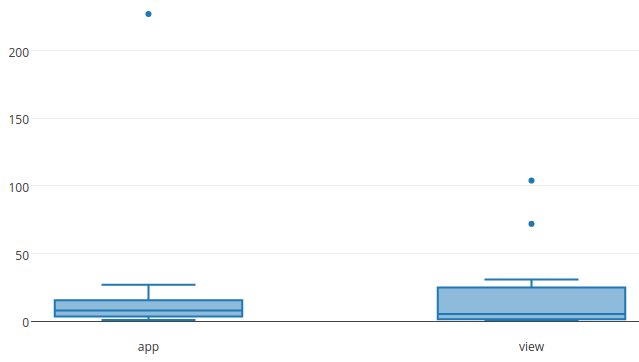
\includegraphics[scale=0.7]{imagens/bloxplot_newapi}
   	\textsf{\caption{Distribuição de ocorrências de NewApi para as taxonomias \textit{app} e \textit{view}}
   	        \label{fig:bloxplot_newapi}}
 \end{figure}


Tais valores refletem o objetivo das taxonomias e a categoria das aplicações.
\textit{App} e \textit{view} contém classes utilizadas em qualquer aplicação, enquanto que a
taxonomia \textit{media} mantém classes relacionadas a multimídia. Mais úteis para um reprodutor
e editor de vídeos (VLC), um navegador web (Firefox) e um aplicativo de comunicação (Telegram)
com recursos de reprodução de multimídia (imagem, som e vídeo) embutido.

A tabela \ref{tab:newapi_app} apresenta os elementos da taxonomia \textit{app} com maior
números de ocorrência de NewApi agrupados pelo elemento de maior granularidade
que surgiu na versão da API indicada por NewApi. Assim, todas as classes do pacote
\texttt{android.app. backup} foram agrupadas pelo pacote porque o próprio pacote
surgiu apenas na versão 5. A classe \texttt{android.app.Fragment} surgiu na versão
11, então agrupamos aqui todos os seus métodos. Já a classe \texttt{android.app.Activity}
existe desde a versão 1 e foram diversos métodos novos apontados por NewApi. Na
classe \texttt{android.app.Notification}, que existe desde a versão 1, apenas o
método \texttt{bigContentView} é apontado por NewApi.

\begin{table}[!htbp]
  \centering
  \caption{Elementos da taxonomia \textit{app} com ocorrências de NewApi}
  \begin{tabular}{| l | r | r |}
  	\hline
  	% rótulo das colunas
  	\multicolumn{1}{|c|}{\textbf{Descrição}} &
  	\begin{tabular}[c]{@{}c@{}}
  	 		\textbf{Ocorrências de}\\ \textbf{NewApi (A)}
  	\end{tabular} &
  	\textbf{Aplicações} \\ \hline
 	%dados
 	\textbf{Classe android.app.Fragment}			& 188 	& 2 \\ \hline
 	Pacote android.app.backup						& 36	& 4 \\ \hline
 	Métodos de android.app.Activity 				& 30 	& 8 \\ \hline
 	Classe android.app.Presentation 				& 28 	& 2  \\ \hline
 	Método android.app.Notification\#bigContentView	& 17 	& 1  \\ \hline
 	Classe android.app.ActionBar  					& 12 	& 3 \\ \hline
 	Classe android.app.Notification.Builder   		& 10 	& 1 \\ \hline
 	\textbf{Classe android.app.FragmentTransaction}	& 9 	& 2  \\ \hline
 	Classe android.app.DownloadManager     			& 9		& 1   \\ \hline
 	\textbf{Classe android.app.FragmentManager}    	& 7		& 2   \\ \hline
  \end{tabular}
  \label{tab:newapi_app}
\end{table}

Da taxonomia \textit{app}, a classe mais comum é \texttt{Fragment}, conforme
apresentado na tabela \ref{tab:newapi_app}. Além disso, alguns métodos da classe
\texttt{Activity} nessa relação são relacionadas aos fragmentos, assim como as
classes \texttt{FragmentTransaction} e \texttt{FragmentManager}. Além dos elementos
apresentados na tabela \ref{tab:newapi_app}, outros 7 elementos possuem um valor
máximo de 4 ocorrências relacionadas.

Se as ocorrências para a taxonomia \textit{app} ficaram concentradas em elementos
relacionados a fragmentos, na taxonomia \textit{view} houve uma maior dispersão.
A classe mais comum, tanto em aplicações (12) quanto em ocorrências de NewApi (108),
é a classe \texttt{View}, classe base para todos os componentes de construção de
interface gráfica. Atributos ou tags XML correspondem a 50 ocorrências, distribuídas
em 7 aplicações. Os demais elementos, aparecem em no máximo 4 aplicações, o que
demonstra serem específico do tipo de aplicação. Por exemplo, as classes
\texttt{InputMethodSubtype} e \texttt{InputMethodManager} juntas somam 12 ocorrências
de NewApi, mas todas elas em uma única aplicação, a AnySoftKeyboard, uma aplicação de
teclado virtual. 

A tabela \ref{tab:newapi_view} apresenta os 10 elementos da taxonomia \textit{view}
com mais ocorrência de NewApi. Além desses, outros 20 elementos apresentam no máximo
6 ocorrências.

\begin{table}[!htbp] % TODO posicionar melhor essa tabela
  \small
  \centering
  \caption{10 elementos da taxonomia \textit{view} com mais ocorrências de NewApi}
  \begin{tabular}{| l | r | r |}
  	\hline
  	% rótulo das colunas
  	\multicolumn{1}{|c|}{\textbf{Descrição}} &
  	\begin{tabular}[c]{@{}c@{}}
  	 		\textbf{Ocorrências}\\ \textbf{de NewApi}
  	\end{tabular} &
 	\textbf{Aplicações} \\ \hline
 	%dados
 	Métodos de android.view.View							& 108 	& 12 \\ \hline
 	Atributos ou tags XML									& 50	& 7 \\ \hline
 	Classe android.view.ViewPropertyAnimator 				& 43 	& 2 \\ \hline
 	Classe android.view.WindowInsets 						& 23 	& 1  \\ \hline
 	Classe android.view.TextureView							& 21 	& 2  \\ \hline
 	Classe android.view.ScaleGestureDetector  				& 12 	& 3 \\ \hline
 	Classe android.view.ActionMode   						& 11 	& 3 \\ \hline
 	Métodos de android.view.MotionEvent						& 10 	& 1  \\ \hline
 	Construtor de android.view.ViewOutlineProvider     		& 10	& 1   \\ \hline
 	Classe android.view.accessibility.AccessibilityNodeInfo & 9		& 1   \\ \hline
  \end{tabular}
  \label{tab:newapi_view}
\end{table}

Tanto os elementos relacionados a fragmentos, quanto a grande maioria dos métodos
da classe \texttt{View} citados anteriormente surgiram na versão 11 da API, e foram
uma importante melhoria na plataforma, o que reforça o alto índice de ocorrências de
NewApi relacionado a esta versão, conforme apresentado no figura \ref{fig:newapi_por_versao}.
Tais ocorrências estão distribuídas em 18 aplicações. 

\begin{figure}[htb]
	\centering 
  	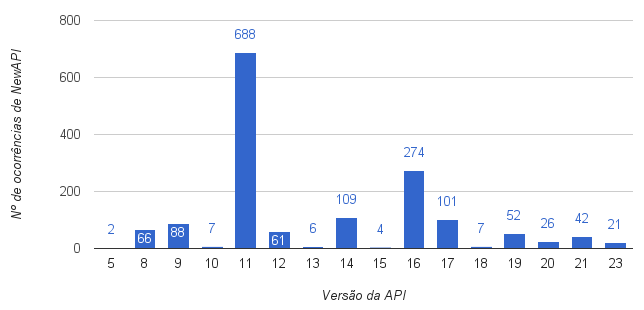
\includegraphics[scale=0.6]{imagens/newapi_por_versao}
  	\textsf{\caption{Nº de ocorrências de NewApi por versão da API}
  	        \label{fig:newapi_por_versao}}
\end{figure}

\subsection{Qual o esforço necessário para aumentar a compatibilidade com um
maior número de APIs de versões anteriores da plataforma?}

Definir um valor de API mínima para execução da aplicação, significa deixar de
atender todos os aparelhos com API inferior. Em algumas situações, isso pode
representar uma perda do mercado potencial. Assim, analisamos qual seria o esforço
para aumentar a compatibilidade com um maior número de APIs. Para tal, editamos o
código-fonte da aplicação (arquivos \texttt{build.gradle} ou \texttt{AndroidManifest.xml},
conforme o caso) e re-executamos o Lint NewApi. Então comparamos o resultado aqui
obtido com o resultado obtido na versão original.

Inicialmente, identificamos a quantidade de novas ocorrências de NewApi que
surgiam com a diminuição da versão da API. Isso fornece um valor quantitativo
do trabalho necessário para aumento da compatibilidade, quanto maior este valor
mais adequações seriam necessárias no código-fonte. A tabela \ref{tab:esforco}
apresenta tais resultados. Para cada aplicação, indicamos situação atual, com
a API mínima atual e a quantidade de ocorrências de NewApi, a situação após nova
edição, com a nova API e a quantidade de ocorrências de NewApi, e a diferença de 
ocorrência de NewApi, com a diferença total de novas ocorrências e dessas a quantidade
de ocorrências únicas. Essas duas últimas colunas mensuram quantitativamente o esforço
necessário para aumentar a compatibilidade.   

% Please add the following required packages to your document preamble:
% \usepackage{multirow}
\begin{table}[!htbp]
\small
\centering
\caption{Esforço quantitativo para aumentar compatibilidade com mais versões da API}
\label{tab:esforco}
\begin{tabular}{|l|r|r|r|r|r|r|}
\hline
\multicolumn{1}{|c|}{\multirow{2}{*}{\textbf{Aplicação}}}                & \multicolumn{2}{c|}{\textbf{Situação atual}}                                                                                                                                       & \multicolumn{2}{c|}{\textbf{Situação após edição}}                                                                                                                                 & \multicolumn{2}{c|}{\textbf{\begin{tabular}[c]{@{}c@{}}Diferenças de\\ ocorrências\\ de NewApi\end{tabular}}}                                                                          \\ \cline{2-7} 
\multicolumn{1}{|c|}{}                                                   & \multicolumn{1}{c|}{\textbf{\begin{tabular}[c]{@{}c@{}}API\\ Mínima\end{tabular}}} & \multicolumn{1}{l|}{\textbf{\begin{tabular}[c]{@{}l@{}}Ocorrências\\ de NewApi\end{tabular}}} & \multicolumn{1}{c|}{\textbf{\begin{tabular}[c]{@{}c@{}}API\\ Mínima\end{tabular}}} & \multicolumn{1}{l|}{\textbf{\begin{tabular}[c]{@{}l@{}}Ocorrências\\ de NewApi\end{tabular}}} & \multicolumn{1}{c|}{\textbf{\begin{tabular}[c]{@{}c@{}}Diferen\\ ça total\end{tabular}}} & \multicolumn{1}{c|}{\textbf{\begin{tabular}[c]{@{}c@{}}Ocorrên\\ cias únicas\end{tabular}}} \\ \hline
\begin{tabular}[c]{@{}l@{}}Numix Circle\\ icon pack\end{tabular}         & 16                                                                                 & 0                                                                                             & 15                                                                                 & 1                                                                                             & 1                                                                                        & 1                                                                                           \\ \hline
SnoopSnitch                                                              & 16                                                                                 & 19                                                                                            & 15                                                                                 & 15                                                                                            & 2                                                                                        & 1                                                                                           \\ \hline
\begin{tabular}[c]{@{}l@{}}Yaaic -\\ IRC Client\end{tabular}             & 21                                                                                 & 0                                                                                             & 15                                                                                 & 1                                                                                             & 1                                                                                        & 1                                                                                           \\ \hline
\begin{tabular}[c]{@{}l@{}}Hangar -\\ Smart app\\ shortcuts\end{tabular} & 16                                                                                 & 14                                                                                            & 15                                                                                 & 21                                                                                            & 7                                                                                        & 5                                                                                           \\ \hline
\begin{tabular}[c]{@{}l@{}}WiFi\\ Analyzer\end{tabular}                  & 22                                                                                 & 0                                                                                             & 21                                                                                 & 1                                                                                             & 1                                                                                        & 1                                                                                           \\ \hline
AcDisplay                                                                & 16                                                                                 & 167                                                                                           & 15                                                                                 & 193                                                                                           & 26                                                                                       & 10                                                                                          \\ \hline
\begin{tabular}[c]{@{}l@{}}Indic\\ Keyboard\end{tabular}                 & 16                                                                                 & 7                                                                                             & 15                                                                                 & 16                                                                                            & 9                                                                                       & 1                                                                                           \\ \hline
Focal                 													 & 16        & 3                                                                     & 15                    & 14                                                                      & 11                                                                                       & 5                                                                                           \\ \hline
\begin{tabular}[c]{@{}l@{}}DashClock\\ Widget\end{tabular}               & 17                                                                                 & 5                                                                                             & 16                                                                                 & 46                                                                                            & 41                                                                                       & 9                                                                                           \\ \hline
Termux                                                                   & 21                                                                                 & 2                                                                                             & 19                                                                                 & 59                                                                                            & 57                                                                                       & 9                                                                                           \\ \hline
\end{tabular}
\end{table}

Posteriormente, analisamos cada uma dessas ocorrências para identificar como ela
poderia ser tratada e qual o impacto para a aplicação. Das 10 aplicações analisadas,
5 delas podem aumentar a compatibilidade com poucos e simples ajustes, fazendo uso
de pacote de compatibilidade e/ou execução condicional, sem perda de funcionalidade.
Quatro dessas aplicações, poderiam passar a exigir API 15, no lugar da atual 16. Mas
uma delas, Yaaic, poderia substituir a API 21 pela API 15, com apenas 1 ocorrência de
NewApi a mais. Tal ocorrência existe devido ao uso do tema Material\cite{Material},
que pode ser tratado através do mecanismos de recursos da plataforma, bastando definir
estilos gerais, para versões inferiores a 21, e um estilo específico (style-v21) para
versão 21 ou superior. Nesta aplicação, também é possível ir além, e prover
compatibilidade com a versão 10 da API. Em que 8 novas ocorrências de NewApi surgiriam,
mas poderiam ser resolvidas com pacote de compatibilidade.

Outras 2 aplicações - Indic Keyboard e AcDisplay - precisam tratar, respectivamente,
9 e 26 novas ocorrências de NewApi para alterar a API de 16 para 15. A primeira teria
que apenas fazer uma re-implementação da classe \texttt{SentenceSuggestionsInfo},
surgida na API 16. Todas as 9 ocorrências de NewApi são referências para essa classe.
A segunda teria que tomar providências diversas, como pacote de compatibilidade, execução
condicional e re-implementação de recursos. Mas todas elas possíveis de resolução sem perda
de funcionalidade na aplicação.

As três aplicações restantes usam funcionalidades mais críticas. Focal, uma
aplicação de fotografia, apresenta um total de 11 ocorrências, sendo que uma
delas parece não haver solução possível, pois depende de suporte do hardware
do aparelho para auto focus da câmera. DashClock Widget apresentou 41 novas
ocorrências ao reduzir a versão da API de 17 para 16. A maioria pode ser
resolvida pelos métodos já citados, 17 delas são referências a classe
\texttt{DreamService}, uma classe específica para realidade virtual.
Portanto, a aplicação poderia fornecer as demais funções mas omitir esta
específica. Por fim, a aplicação Termux, um emulador de terminal, é a que
possui a maior quantidade de ocorrências de NewApi, ao reduzir a versão da
API de 21 para 19: 57 ocorrências. A maioria facilmente tratada pelos métodos
já citados. Porém, 9 delas fizerem referência a classe \texttt{android.system.Os},
as quais são funcionalidades fundamentais para a aplicação, de acesso ao sistema.
Distribuir a aplicação sem tais recursos seria uma perda considerável. Essa classe
expõe para a API pública do Android uma classe pertencente ao pacote \texttt{libcore},
o qual não pode ser importado pelas classes das aplicações da mesmo forma que classes
do pacote \texttt{android}. No entanto, é possível através de uma re-implementação de
recurso mais elaborada que as citadas anteriormente, usando reflexão, acessar tal pacote
e classes internas \cite{Libcore}, e então fazer uma implementação própria da classe \texttt{Os},
ainda que fazer uso de APIs internas seja uma má prática de programação e existam
recomendações contrárias à sua adoção \cite{Businge2015} \cite{Mastrangelo2015}.

A tabela \ref{tab:esforco_resumo} resume o resultado qualitativo, agrupando as aplicações
em três níveis de dificuldade e possíveis soluções para as novas ocorrências de NewApi.
Os níveis de dificuldade foram definidos da seguinte forma:
\begin{enumerate}
	\item Baixo: necessário apenas uso de pacote de compatibilidade, execução condicional ou
	uso de estilo especializado;
	\item Médio: necessário re-implementação simples de recurso. Pode-se, por exemplo, copiar
	classes do código-fonte da API;
	\item Alto: necessário alguma implementação de recurso mais elaborada ou ausência do
	recurso em aparelhos com API mais antiga. Deve-se, por exemplo, usar reflexão para
	ter acesso à API interna.
\end{enumerate}
Os resultados encontrados, associado à tabela de distribuição das versões (figura 
\ref{fig:platform_versions}), apresenta evidências de que as aplicações poderiam,
com um esforço de baixo a médio, aumentar a compatibilidade com um maior número de
versões da API.  

% Please add the following required packages to your document preamble:
% \usepackage{multirow}
\begin{table}[!htbp]
\centering
\caption{Nível de dificuldade para aumentar a compatibilidade e possíveis soluções
para as novas ocorrências de NewApi}
\label{tab:esforco_resumo}
\begin{tabular}{|l|c|l|l|l|}
\hline
\multicolumn{1}{|c|}{\multirow{2}{*}{\textbf{Aplicação}}}                & \multicolumn{2}{c|}{\multirow{2}{*}{\textbf{\begin{tabular}[c]{@{}c@{}}Nível de\\ Dificuldade\end{tabular}}}} & \multicolumn{2}{c|}{\multirow{2}{*}{\textbf{\begin{tabular}[c]{@{}c@{}}Possíveis\\ Soluções\end{tabular}}}}                                                                                     \\
\multicolumn{1}{|c|}{}                                                   & \multicolumn{2}{c|}{}                                                                                         & \multicolumn{2}{c|}{}                                                                                                                                                                           \\ \hline
\begin{tabular}[c]{@{}l@{}}Numix Circle\\ icon pack\end{tabular}         & \multicolumn{2}{c|}{\multirow{5}{*}{Baixo}}                                                                   & \multicolumn{2}{l|}{\multirow{5}{*}{\begin{tabular}[c]{@{}l@{}}- Execução condicional\\ - Pacote de compatibilidade\\ - Uso de estilo especializado\end{tabular}}}                              \\ \cline{1-1}
SnoopSnitch                                                              & \multicolumn{2}{c|}{}                                                                                         & \multicolumn{2}{l|}{}                                                                                                                                                                           \\ \cline{1-1}
\begin{tabular}[c]{@{}l@{}}Yaaic -\\ IRC Client\end{tabular}             & \multicolumn{2}{c|}{}                                                                                         & \multicolumn{2}{l|}{}                                                                                                                                                                           \\ \cline{1-1}
\begin{tabular}[c]{@{}l@{}}Hangar -\\ Smart app\\ shortcuts\end{tabular} & \multicolumn{2}{c|}{}                                                                                         & \multicolumn{2}{l|}{}                                                                                                                                                                           \\ \cline{1-1}
\begin{tabular}[c]{@{}l@{}}WiFi\\ Analyzer\end{tabular}                  & \multicolumn{2}{c|}{}                                                                                         & \multicolumn{2}{l|}{}                                                                                                                                                                           \\ \hline
AcDisplay                                                                & \multicolumn{2}{c|}{\multirow{2}{*}{Médio}}                                                                   & \multicolumn{2}{l|}{\multirow{2}{*}{\begin{tabular}[c]{@{}l@{}}- Algumas ocorrências são ignoradas (atributos XML) \\ - Pacote de Compatibilidade\\ - Reimplementação de recurso\end{tabular}}} \\ \cline{1-1}
\begin{tabular}[c]{@{}l@{}}Indic\\ Keyboard\end{tabular}                 & \multicolumn{2}{c|}{}                                                                                         & \multicolumn{2}{l|}{}                                                                                                                                                                           \\ \hline
Focal (Beta)                                                             & \multicolumn{2}{c|}{\multirow{3}{*}{Alto}}                                                                    & \multicolumn{2}{l|}{\multirow{3}{*}{\begin{tabular}[c]{@{}l@{}}- Pacote de compatibilidade\\ - Reimplementação de recurso\\ - Execução condicional\\ - Versão sem recurso\end{tabular}}}        \\ \cline{1-1}
\begin{tabular}[c]{@{}l@{}}DashClock\\ Widget\end{tabular}               & \multicolumn{2}{c|}{}                                                                                         & \multicolumn{2}{l|}{}                                                                                                                                                                           \\ \cline{1-1}
Termux                                                                   & \multicolumn{2}{c|}{}                                                                                         & \multicolumn{2}{l|}{}                                                                                                                                                                           \\ \hline
\end{tabular}
\end{table}

\subsection{Qual a incidência de código morto em função da versão da API do Android?}

A técnica básica de prover suporte a multi-versões da API é o uso de execução
condicional avaliando a versão da API do aparelho. Também faz parte da evolução
natural das aplicações o fim de suporte a versões da API mais antigas. Dessa forma,
é possível que os desenvolvedores alterem a configuração de API mínima no 
\texttt{AndroidManifest.xml}, mas deixem ao longo do código-fonte da aplicação
trechos de código que seriam executados apenas em versões de API inferiores a esta. Nessa
situação, tais trechos de códigos são caracterizados como código-morto.

Para esta questão de pesquisa, foram analisadas 7 aplicações e foi encontrado
código-morto em 4 delas. No entanto, em um valor proporcional muito pequeno em
relação ao total de linhas de código da aplicação. Mesmo considerando apenas o
código Java, identificamos uma média de apenas 0,09\% de linhas de código-morto.
A tabela \ref{tab:codigo_morto} apresenta detalhes dessa análise. São exibidos
as métricas de número de arquivos e total de linhas de código-fonte tanto com
código-morto quanto com a remoção do código morto, assim como a diferença em
valores absolutos e percentuais. 

% Please add the following required packages to your document preamble:
% \usepackage{multirow}
\begin{table}[!htbp]
\caption{Ocorrências de código morto (CM) por aplicação}
\footnotesize
\centering
\label{tab:codigo_morto}
\begin{tabular}{lrrrrrrr|r|r|r|}
\hline
\multicolumn{1}{|c|}{\multirow{2}{*}{\textbf{Aplicação}}}                           & \multicolumn{2}{c|}{\textbf{\begin{tabular}[c]{@{}c@{}}Métricas\\ COM CM\end{tabular}}}                               & \multicolumn{2}{c|}{\textbf{\begin{tabular}[c]{@{}c@{}}Ocorrências\\ de CM\end{tabular}}}                            & \multicolumn{2}{c|}{\textbf{\begin{tabular}[c]{@{}c@{}}Métricas\\ SEM CM\end{tabular}}}                               & \multicolumn{2}{c|}{\textbf{Diferenças}}                                                                                & \multicolumn{2}{c|}{\textbf{Percentuais}}                                                                                \\ \cline{2-11}
\multicolumn{1}{|c|}{}                                                              & \multicolumn{1}{c|}{\textbf{\begin{tabular}[c]{@{}c@{}}Arqui\\ vos\end{tabular}}} & \multicolumn{1}{c|}{\textbf{LoC}} & \multicolumn{1}{c|}{\textbf{\#}} & \multicolumn{1}{c|}{\textbf{\begin{tabular}[c]{@{}c@{}}Arqui\\ vos\end{tabular}}} & \multicolumn{1}{c|}{\textbf{\begin{tabular}[c]{@{}c@{}}Arqui\\ vos\end{tabular}}} & \multicolumn{1}{c|}{\textbf{LoC}} & \multicolumn{1}{c|}{\textbf{\begin{tabular}[c]{@{}c@{}}Arqui\\ vos\end{tabular}}} & \multicolumn{1}{c|}{\textbf{LoC}}   & \multicolumn{1}{c|}{\textbf{\begin{tabular}[c]{@{}c@{}}Arqui\\ vos\end{tabular}}} & \multicolumn{1}{c|}{\textbf{LoC}}    \\ \hline
\multicolumn{1}{|l|}{RingDroid}                                                     & \multicolumn{1}{r|}{12}                                                           & \multicolumn{1}{r|}{4189}         & \multicolumn{1}{r|}{}            & \multicolumn{1}{r|}{}                                                             & \multicolumn{1}{r|}{\textbf{}}                                                    & \multicolumn{1}{r|}{\textbf{}}    & \textbf{}                                                                         & \textbf{}                           & \textbf{}                                                                         & \textbf{}                            \\ \hline
\multicolumn{1}{|l|}{\begin{tabular}[c]{@{}l@{}}Orbot Proxy\\ com Tor\end{tabular}} & \multicolumn{1}{r|}{86}                                                           & \multicolumn{1}{r|}{11147}        & \multicolumn{1}{r|}{3}           & \multicolumn{1}{r|}{3}                                                            & \multicolumn{1}{r|}{86}                                                           & \multicolumn{1}{r|}{11132}        & 0                                                                                 & 15                                  & 0,00\%                                                                            & 0,13\%                               \\ \hline
\multicolumn{1}{|l|}{Transdrone}                                                    & \multicolumn{1}{r|}{243}                                                          & \multicolumn{1}{r|}{23464}        & \multicolumn{1}{r|}{}            & \multicolumn{1}{r|}{}                                                             & \multicolumn{1}{r|}{}                                                             & \multicolumn{1}{r|}{}             &                                                                                   &                                     &                                                                                   &                                      \\ \hline
\multicolumn{1}{|l|}{\begin{tabular}[c]{@{}l@{}}Vanilla\\ Music\end{tabular}}       & \multicolumn{1}{r|}{90}                                                           & \multicolumn{1}{r|}{17404}        & \multicolumn{1}{r|}{3}           & \multicolumn{1}{r|}{1}                                                            & \multicolumn{1}{r|}{90}                                                           & \multicolumn{1}{r|}{17398}        & 0                                                                                 & 6                                   & 0,00\%                                                                            & 0,03\%                               \\ \hline
\multicolumn{1}{|l|}{AFWall+}                                                       & \multicolumn{1}{r|}{84}                                                           & \multicolumn{1}{r|}{14560}        & \multicolumn{1}{r|}{4}           & \multicolumn{1}{r|}{4}                                                            & \multicolumn{1}{r|}{84}                                                           & \multicolumn{1}{r|}{14540}        & 0                                                                                 & 20                                  & 0,00\%                                                                            & 0,14\%                               \\ \hline
\multicolumn{1}{|l|}{aMetro}                                                        & \multicolumn{1}{r|}{133}                                                          & \multicolumn{1}{r|}{8167}         & \multicolumn{1}{r|}{}            & \multicolumn{1}{r|}{}                                                             & \multicolumn{1}{r|}{}                                                             & \multicolumn{1}{r|}{}             &                                                                                   &                                     &                                                                                   &                                      \\ \hline
\multicolumn{1}{|l|}{K-9 Mail}                                                      & \multicolumn{1}{r|}{484}                                                          & \multicolumn{1}{r|}{78984}        & \multicolumn{1}{r|}{8}           & \multicolumn{1}{r|}{8}                                                            & \multicolumn{1}{r|}{484}                                                          & \multicolumn{1}{r|}{78934}        & 0                                                                                 & 50                                  & 0,00\%                                                                            & 0,06\%                               \\ \hline
                                                                                    & \multicolumn{1}{l}{}                                                              & \multicolumn{1}{l}{}              & \multicolumn{1}{l}{}             & \multicolumn{1}{l}{}                                                              & \multicolumn{1}{l}{}                                                              & \multicolumn{1}{l}{}              & \multicolumn{1}{l|}{}                                                             & \multicolumn{1}{l|}{\textbf{Média}} & \textbf{0,00\%}                                                                   & \multicolumn{1}{l|}{\textbf{0,09\%}} \\ \cline{9-11} 
\end{tabular}
\end{table}

Tais resultados apresentam indícios que é possível encontrar código-morto em aplicações
Android existentes. No entanto, em comparação com a quantidade de linhas de código total
da aplicação, a quantidade de linhas de código morto é irrelevante, conforme mostra a
tabela \ref{tab:codigo_morto}.

\section{Discussão} \label{sec:discussao}

Os dados coletados no estudo de caso e as análises realizadas nas seções anteriores
são fonte de evidências para a constatação das hipóteses. Cada questão de pesquisa
será abordada separadamente a seguir, juntamente com sua hipótese relacionada.

\subsection{Quais são as técnicas que aplicações atuais usam para manter compatibilidades
com as diversas versões da API do Android?} \label{subsec:tecnicas}

\begin{itemize}
	\item \textbf{Proposição P1}: Se a plataforma oferece suporte para múltiplas versões
	da API e tal suporte tem impacto no mercado em potencial então os desenvolvedores
	utilizam tal recurso.
	\item \textbf{Hipótese H1}: As aplicações utilizam pelo menos uma das técnicas disponíveis
	para oferecer suporte a múltiplas versões da API.
\end{itemize}

No nosso estudo, das 25 aplicações analisadas: (i) apenas 2 utilizam uma única
estratégia, (ii) 9 aplicações utilizam 2 estratégias; e (iii) 13 fazem uso das
3 estratégias diferentes. Finalmente, apenas a aplicação \textit{Shattered Pixel
Dungeon}, um jogo de RPG, não utilizou nenhuma dessas soluções. Portanto, é a
única que exige uma baixa API para instalação (versão 8) sem se preocupar com
o uso de recursos mais modernos. Seja através de uso explícito da nova API,
quando estiverem disponíveis, seja adicionando a dependência ao pacote de
compatibilidade ou da re-implementações de recursos, quando seria possível
usar novos recursos mesmo em versões mais antigas da API, 96\% das aplicações
analisadas utilizam pelo menos uma técnica para oferecer suporte a múltiplas
versões da API. Portanto, tais resultado oferecem elementos
para validar a hipótese \textbf{H1}. A seguir, discutiremos características de cada
uma dessas formas de implementação de suporte a múltiplas versões da API.

\subsubsection{Pacote de compatibilidade}
O uso do pacote de compatibilidade oficial foi a forma mais comum para prover
suporte aos dispositivos com versões antigas, sendo utilizada por 23 das 25
aplicações analisadas. A tabela \ref{tab:fw_pacote} apresenta as características
do pacote de compatibilidade segundo o framework de comparação apresentado na
seção \ref{sec:framework}.

\begin{table}[!htbp]
  \centering	
  \caption{Descrição do pacote de compatibilidade segundo o framework de comparação}
  \label{tab:fw_pacote}
  \begin{tabular}{ | l | l |}
    \hline
    \textbf{Critério de avaliação} 	& \textbf{Valores obtido}  \\ \hline
    Tipo de variabilidade 			& Ambos  \\ \hline
    Variabilidade na estrutura 		& Oferece suporte \\ \hline
    Variabilidade no comportamento 	& Oferece suporte \\ \hline
    Granularidade 					& Grossa \\ \hline
    Tempo de ligação 				& Compilação \\ \hline
    Reusabilidade 					& Alta \\ \hline
    Legibilidade 					& Baixo impacto \\ \hline
    Tamanho da aplicação 			& Médio impacto \\ \hline
  \end{tabular}
\end{table}

Pacotes de compatibilidade substituem de forma estática componentes de versões
anteriores da API por componentes de novas versões, de forma que oferece suporte
para o tipo de variabilidades positivas e negativas. Também oferece suporte à
granularidade grossa, já que os componentes são substituídos por completo. Tal
substituição equivale tanto a adicionar quanto a remover métodos e atributos nas
classes, ou sobrescrever os existentes, portanto, essa técnica oferece suporte para
variabilidade na estrutura e no comportamento. Essa técnica também exerce um baixo
impacto na legibilidade do código e no desempenho da aplicação. Uma vez que, na maioria
dos casos, basta alterar a importação das classes, como mostramos  na Seção \ref{subsec:pacote-compatibilidade}.
No entanto, pode resultar em um aumento no tamanho
da aplicação, ou no caso particular do Android, um estouro no limite de métodos das
aplicações \cite{Estouro}, já que o tempo de ligação dessa técnica é durante a compilação
e mais elementos serão empacotados juntamente com a aplicação.

\subsubsection{Re-implementação de Recursos}
Os resultados do critérios de avaliação dessa técnica, apresentados na tabela
\ref{tab:fw_reimplementacao}, são semelhantes aos do pacote de compatibilidade.
Diferenciando em três critérios apenas: i) reusabilidade; ii) legibilidade e;
iii) tamanho da aplicação. A reusabilidade é alta em relação à própria aplicação,
mas baixa em relação a outras aplicações. Legibilidade é prejudicada por aumentar
a quantidade de pacotes e classes na aplicação. Esses dois aspectos podem ser
melhorados convertendo esse conjunto de classes em um projeto separado, sendo
integrado à aplicação da mesma forma que pacotes de compatibilidade. No entanto,
como a re-implementação é feita apenas do que será utilizado, o impacto no tamanho
da aplicação é menor, em relação ao pacote de compatibilidade. 

\begin{table}[!htbp]
  \centering	
  \caption{Descrição da re-implementação de recurso segundo o framework de comparação}
  \label{tab:fw_reimplementacao}
  \begin{tabular}{ | l | l |}
    \hline
    \textbf{Critério de avaliação} 	& \textbf{Valores obtido}  \\ \hline
    Tipo de variabilidade 			& Ambos  \\ \hline
    Variabilidade na estrutura 		& Oferece suporte \\ \hline
    Variabilidade no comportamento 	& Oferece suporte \\ \hline
    Granularidade 					& Grossa \\ \hline
    Tempo de ligação 				& Compilação \\ \hline
    Reusabilidade 					& Médio \\ \hline
    Legibilidade 					& Médio impacto \\ \hline
    Tamanho da aplicação 			& Baixo impacto \\ \hline
  \end{tabular}
\end{table}

A recomendação é evitar o uso de pacotes de compatibilidades quando o que será
utilizado é muito pouco \cite{Estouro}. O que pode ser feito por meio da técnicas
de re-implementação do recurso, como realizado por 14 aplicações do nosso estudo.
Além de evitar o aumento de métodos da aplicação que não serão utilizados, será
possível uma maior personalização do comportamento dos componentes. No entanto,
é um elemento a mais que os desenvolvedores deverão se preocupar em evoluir
juntamente com o restante da aplicação. Diferentemente dos pacotes de compatibilidade,
cuja evolução é feita por equipes dedicadas e externas ao projeto.

Um outro problema de re-implementação de recursos, este não-técnico mas legal,
diz respeito a licença de uso de código alheio. É comum a re-implementação de
recursos ser feita por simples cópia dos arquivos úteis de outros projetos já
existentes, o que pode acarretar problemas legais e que são subestimados pelos
desenvolvedores \cite{Minelli}.

\subsubsection{Uso explícito da nova API}
Uso explícito da nova API foi apontado pelo Android Lint em 22 aplicações. Tais
ocorrências devem possuir alguma forma de proteção às chamadas para serem executados
apenas em dispositivos com a nova versão da API.  Foram identificadas diversas formas
de proteção: execução condicional direta e indireta, padrões de projeto, suporte implícito,
métodos nunca executadas. Além de situações em que a chamada não está protegida, portanto,
a aplicação está suscetível a erros durante a execução.  A seguir, tais soluções de projeto
são discutidas.

\paragraph{Execução condicional}

Execução condicional, direta ou indireta, foi observado em 18 aplicações.
A tabela \ref{tab:fw_EC} descreve essa técnica segundo o framework de
comparação apresentado na seção \ref{sec:framework}.

\begin{table}[!htbp]
  \centering	
  \caption{Descrição do padrão execução condicional segundo o framework de comparação}
  \label{tab:fw_EC}
  \begin{tabular}{ | l | l |}
    \hline
    \textbf{Critério de avaliação} 	& \textbf{Valores obtido}  \\ \hline
    Tipo de variabilidade 			& Negativo  \\ \hline
    Variabilidade na estrutura 		& Não oferece suporte \\ \hline
    Variabilidade no comportamento 	& Oferece suporte \\ \hline
    Granularidade 					& Fina, Grossa \\ \hline
    Tempo de ligação 				& Execução \\ \hline
    Reusabilidade 					& Baixa \\ \hline
    Legibilidade 					& Alto impacto \\ \hline
    Tamanho da aplicação 			& Baixo impacto \\ \hline
  \end{tabular}
\end{table}

EC oferece suporte apenas para variabilidade do tipo negativa. Com EC é possível,
com o condicional, remover trechos de código da execução, mas não adicionar. Uma
vez que o tempo de ligação é durante a  execução, essa técnica não oferece suporte
para variabilidade na estrutura, apenas no comportamento. E, apesar do tempo de
ligação ser na execução, o que pode implicar em repetidos desvios condicionais,
o impacto no desempenho é baixo, graças ao mecanismo do repositório de parâmetros,
que apenas obtém o valor de um atributo estático de uma classe.

EC pode definir o tipo dos objetos a serem criados, oferecendo suporte à granularidade
grossa, ou apenas a execução ou não de uma linha de código qualquer, dando suporte à
granularidade fina. No último caso, que é mais comum,  reusabilidade e legibilidade
são prejudicadas. 

Para verificar o impacto no tamanho da aplicação, realizamos uma grande refatoração
em uma das aplicações, o Telegram. Eliminamos todas as EC parametrizadas com a versão
da API, deixando o mesmo com suporte apenas para a versão 23 da plataforma, além de
outros artefatos como imagens e arquivos de layout. Um total de 145 arquivos foram 
editados ou
apagados. Comparando os tamanhos dos arquivos APK's dessa versão e da versão com suporte
a partir da API 9 não foi verificada diferença alguma. Portanto, essa técnica tem baixo
impacto no tamanho das aplicações.

Apesar de execução condicional trazer uma baixa legibilidade no código, seu uso
é bastante simples e comum, não exigindo conhecimentos avançados e nem uso de
ferramentas externas, como exige a técnica de 
\abrv[CC -- \textit{Compilação Condicional}]
{compilação condicional}(CC)
\cite{Medeiros2015}. A técnica de CC é bastante utilizada em outras plataformas
para gerência de variabilidades \cite{Liebig2010}, entretanto não foi observado
seu uso em nenhuma das aplicações analisadas no nosso estudo. Dois fatores podem
contribuir para a baixa legibilidade: (i) o código de todas as variabilidades
estarão presentes em todos produtos da LPS; (ii) uso de \texttt{Build.VERSION\_CODES}.
O primeiro é intrínseco ao padrão, já o segundo é específico da plataforma Android.
A classe \texttt{Build.VERSION\_CODES} contém atributos que mapeiam a versão da API.
Quando eles são utilizados no código, frequentemente é necessário recorrer à tabela
presente na figura \ref{fig:platform_versions}. Além disso, quando a execução
condicional é indireta pode existir uma grande distância entre o código da condição
e o código efetivamente da variação da plataforma. Isso pode facilitar a inclusão de
novos acessos a essa linha de código sem passar pela condição, portanto, execução
condicional indireta deve ser utilizado com cuidado e estar bem documentado.

\paragraph{Padrões de Projeto}
Execução condicional é uma forma primitiva de modularização. Padrões de projeto
podem ser utilizados para melhorar a modularização. Alguns deles foram identificados
nas aplicações. A tabela \ref{tab:fw_padroes} sintetiza a análise de tais padrões de
projeto segundo o framework de comparação.

\begin{table}[!htbp]
  \centering	
  \caption{Descrição dos padrões de projeto utilizados nas aplicações analisadas}
  \label{tab:fw_padroes}
  \begin{tabular}{ | l | l |}
    \hline
    \textbf{Critério de avaliação} 	& \textbf{Valores obtido}  				\\ \hline
    Tipo de variabilidade 			& Ambos (Strategy, Null Object, Proxy)   \\ \hline
    Variabilidade na estrutura 		& Não oferece suporte 					\\ \hline
    Variabilidade no comportamento 	& \begin{tabular}[c]{@{}l@{}}
            						  Oferece suporte (Strategy, Null Object,\\
            						  Proxy)
            						  \end{tabular}									 \\ \hline
    Granularidade 					& Grossa (Strategy, Proxy), Fina (Null Object)   \\ \hline
    Tempo de ligação 				& \begin{tabular}[c]{@{}l@{}}
        								Execução (Strategy, Null Object),\\
        								Compilação (Proxy)
        							\end{tabular}								 	\\ \hline
    Reusabilidade 					& Alta (Strategy, Null Object) 					\\ \hline
    Legibilidade 					&  \begin{tabular}[c]{@{}l@{}}
    										Baixo impacto (Strategy), Médio impacto\\
    										(Proxy), Alto impacto (Null Object)
    									\end{tabular}								 \\ \hline
    Tamanho da aplicação 			& Médio impacto (Strategy, Null Object, Proxy)  \\ \hline
   \end{tabular}
\end{table}

Como alguns padrões de projeto foram identificados, é necessário que a avaliação
seja feita separadamente. Cada padrão possui suas propriedades. O padrão
\textit{Proxy} utilizado levou a uma grande dispersão do código verificador da
necessidade do proxy, ocorrendo dentro de todos os métodos do próprio proxy.
\textit{Proxy} foi utilizado em situações em que não é possível controlar a criação
dos objetos, que é feita pela própria plataforma. Em particular, foi comum para
tratar evoluções da classe \texttt{View}.

A solução adotada pela aplicação AnkiDroid ao utilizar o padrão \textit{Strategy}
mostrou-se bastante efetiva, onde cada classe que representa uma "estratégia concreta"
implementa especificamente os métodos que sofreram alteração entre as versões, herdando
os demais métodos das versões imediatamente anterior. A aplicação K-9 Mail também utilizou
\textit{Strategy}, mas não há relação de herança entre as classes "estratégia" e elas são
somente duas.

O padrão \textit{Strategy} também poderia ter sido utilizado na aplicação C:geo,
no entanto, foi escolhido o padrão \textit{Null Object}. Essa solução é de baixa
legibilidade, sendo necessária a implementação de 3 elementos para cada versão da
API a ser oferecido suporte: uma interface com os métodos, uma classe que implementa
essa interface, e outra que também implementa, mas os seus métodos nada fazem, é o
\textit{"null object"}. Além disso, como as interfaces são diferentes, não é possível
usar polimorfismo, e a programação é específica para cada implementação, demonstrando
assim ser uma solução difícil de manter. Atualmente, 3 versões foram suportadas:
11, 13 e 19.

\paragraph{Suporte Implícito}

Algumas ocorrências de chamadas a nova API estão dentro de métodos da própria API
adicionados também nas novas versões e que são executados de forma automática pela
própria plataforma. Portanto, a chamada está implicitamente protegida. Outra situação
onde ocorre essa forma de proteção é no uso de elementos XML, que embora sejam apontados
pelo Lint NewApi, a plataforma só irá executá-los em versões superiores àquele da adição
do elemento. 

Esse mecanismo dispensa o uso de execução condicional. No entanto, pode dificultar o
entendimento por parte da equipe de desenvolvimento, dado que os desenvolvedores deverão
ter o conhecimento de quais versões da API permitirá a execução de determinados métodos.

\subsubsection{Quando as Técnicas Foram Utilizadas}

Foram detectados alguns padrões de uso dos mecanismos para manter compatibilidades com
as diversas versões da API do Android. Pacote de compatibilidade é utilizado quando se
deseja um conjunto de novos recursos, cujo implementação está distribuída em diversos
arquivos, como as APIs de fragmentos e barra de ação.

Re-implementação de recursos é utilizado para situações pontuais. Quando o código do
recurso desejado está localizado em uma classe apenas, como a \texttt{Base64},  ou
várias mas organizadas em um único pacote da API, como \texttt{android.animation}.
Também é utilizada para situações em que o recurso não está disponível nos pacotes
de compatibilidade.

Pacote de compatibilidade e re-implementação de recursos são utilizadas para uso de
recursos de granularidade grossa, a partir de classes. Para casos de granularidade
fina, quando o recurso desejado são métodos de classes já existentes em versões
anteriores, usa-se execução condicional direta ou indireta.

Com o objetivo de concentrar as ocorrências às chamadas da nova API, evitando o
espalhamento de instruções condicionais ao longo do código, pode-se utilizar algum
padrão de projeto. No entanto, com exceção do padrão de projeto \textit{Proxy},
não foram determinados os motivos de uso de um ou outro padrão, ficando a cargo da
escolha de individual de cada desenvolvedor. O padrão de projeto \textit{Proxy} foi
utilizado em situações em que a instanciação do objeto é feito pela própria plataforma,
como objetos da classe \texttt{View}.

Também é importante destacar que os próprios pacotes de compatibilidade exigem uma
versão mínima de API. Os nomes dos pacotes possuem em sua composição um trecho v\#,
que representa a versão mínima exigida por ele \cite{SupportLibrary2017}. 
Por exemplo, os pacotes support-v4 e appcompat-v7 exigem, respectivamente, API 4 e
API 7\footnote{Recentemente (agosto de 2016), houve uma mudança nesse política e
as versões dos pacotes superiores a 24.2.0 passaram a exigir API nível 9 para todos
os pacotes. Por essa razão, os pacotes support-v4 e support-v7 exigem API mínima nível
9 para versões do pacote iguals ou superiores a 24.2.0}. Este será um pré-requisito a
ser considerado pelos desenvolvedores no uso dos mecanismos. Neste caso, deverão avaliar
entre aumentar a versão da aplicação, e deixar de atender uma parcela do mercado, utilizar
execução condicional, ou re-implementar os recursos. Nessa última opção, possivelmente será
necessária também a re-implementação do recurso da API utilizada pelo pacote, o que pode
impactar negativamente no esforço necessário.   

\subsection{Qual o subconjunto de novas funcionalidades da plataforma que são mais
utilizados por aplicações compatíveis com versões antigas da API?} \label{subsec:mudancas}

\begin{itemize}
	\item \textbf{Proposição P2}: Se a cada nova versão da plataforma são disponibilizados
	diversos novos recursos então deve existir um subconjunto que é mais utilizado no 
	contexto de suporte a múltiplas versões da API.
	\item \textbf{Hipótese H2}: Existe um subconjunto dos novos recursos da API que é
	mais utilizado no contexto de suporte a múltiplas versões da API.
\end{itemize}

Para determinar o subconjunto de novas funcionalidades da plataforma que são mais
utilizados por aplicações compatíveis com versões antigas da API fizemos a análise
a partir da técnica usada para facilitar portabilidade para novas plataformas: pacote
de compatibilidade, re-implementação de recursos e uso explícito da nova API.

Unificando os três resultados,  os elementos mais utilizados são do pacote
\texttt{android. animation} e classes relacionadas a API de fragmentos, ambas
da versão 11 da API. Isso comprova a importância dessa versão da API para a
plataforma. 

O pacote \texttt{android.animation} fornece mecanismo para animação de propriedades
de qualquer objeto. Com isso, é possível criar efeitos visuais, úteis para uma boa
experiência do usuário, assim como fundamentais em aplicações de jogos. A API de
fragmentos permite o reaproveitamento de pedaços de telas na composição das atividades,
o que é muito útil considerando a diversidade de aparelhos que oferecem suporte para
Android, motivo pelo qual acreditamos ser este um dos elementos mais utilizados. 

A forma principal de uso do pacote \texttt{android.animation} foi através de
re-implemen- tação de recurso, fornecida pelo projeto NineOldAndroids\footnote{http://nineoldandroids.com/},
ou execução condicional. Já a API de fragmentos por pacote de compatibilidade.
Essa distinção se dá pelo fato de que a API de fragmentos fornece classes bases,
em particular \texttt{Fragment}, que deverão ser utilizadas por herança, o que não
permite a composição em tempo de execução. Enquanto os elementos de animação pode
ser instanciados dinamicamente, o que permite utilizar execução condicional.
Atualmente, os elementos de animação são disponibilizados no pacote de compatibilidade,
permitindo que a re-implementa- ção de recurso seja substituída por esse mecanismo.
Tais resultados apresentam evidências suficientes para validarmos a hipótese \textbf{H2}.

\subsection{Qual o esforço necessário para aumentar a compatibilidade com um maior
número de APIs de versões anteriores da plataforma?} \label{subsec:esforco}

\begin{itemize}
	\item \textbf{Proposição P3}: Se as aplicações utilizam apenas APIs mais recentes,
	não possuindo um histórico de uso de APIs antigas, então elas foram desenvolvidas
	sem a preocupação de oferecer suporte às versões antigas da API o que, possivelmente,
	a leva a perder uma fatia do mercado de aplicações.
	\item \textbf{Hipótese H3}: As aplicações podem aumentar o seu mercado potencial com
	baixo esforço em termos de desenvolvimento (alterações em seu código-fonte).
\end{itemize}

A falta de compatibilidade com múltiplas versões da API acarreta uma perda de uma
parcela do mercado potencial. Para aumentar esse mercado é necessário editar a API
mínima exigida para a aplicação e proteger eventuais ocorrências de NewApi que surjam.

Em termos quantitativos, 5 aplicações (50\%) apresentararm menos de 10 novas ocorrências 
de NewApi ao reduzir a versão mínima da API. No geral, surgem, em média, 15,60 novas
ocorrências, considerando a redução para a imediatamente inferior à atual. O caso mais
extremo, que mais se beneficiaria com um menor esforço, é o aplicativo Yaac. Este aplicativo
poderia reduzir sua API mínima de 21 para 15 com o ajuste de apenas uma ocorrência de NewApi.
Indo mais além, poderia reduzir para API 10, com outras 8 ocorrências de NewApi a serem tratadas.

Em termos qualitativos, mesmo nas aplicações mais dependentes de novas APIs, o suporte
poderia ser ampliado usando uma das técnicas discutidas neste trabalho. Tais resultados
apresentam evidências suficientes para validarmos a hipótese \textbf{H3}. 

\subsection{Qual a incidência de código morto em função da versão da API do Android?} 
\label{subsec:codigo_morto}

\begin{itemize}
	\item \textbf{Proposição P4}: Se as aplicações utilizam execução condicional para
	execução de determinados trechos de códigos e a sua API mínima exigida é superior
	à necessária para execução do trecho de código, então tal trecho de código é código-morto.   
	\item \textbf{Hipótese H4}: As aplicações possuem código-morto, que só seriam executados
	na presença de APIs antigas.
\end{itemize}

A hipótese de uma alta incidência de código-morto devido ao suporte a
múltiplas versão da API (\textbf{H4}) não foi confirmada. Embora tenhamos encontrado
código-morto em 4 de 7 aplicações analisadas, a quantidade percentual de linhas de
código é muito baixa,
menos de 0,1\%. Estudos mais detalhados seriam necessários para determinar a causa
disso. No entanto, acreditamos que o uso de padrões de projeto, que permitem uma melhor
coesão do código, favoreçam tal cenário, fazendo com o que o desenvolvedor tenha uma melhor
percepção do código legado que ele deve remover já que não pretende mais atender versões
antigas ou mesmo depender da ajuda de analisadores estáticos como o Lint. Enquanto que
execução condicional pode dificultar a remoção desses códigos durante a evolução da
aplicação, dado existir um maior espalhamento de código.

\section{Ameaças à Validade} \label{sec:ameacas}

Nesta subseção, destacamos algumas ameaças à validade do estudo. Identificá-las
previamente pode minimizar seus efeitos.  Em alguns casos, tais ameaças geram
limitações do estudo que devem ser observadas e corrigidas em trabalhos futuros.

\textbf{Análise manual.} Embora tenhamos utilizado o Lint e desenvolvido um simples
analisador estático, a maior parte das análises foi feita de forma manual. O que
dificultou a determinação de padrões de projeto e ocorrências de execuções condicionais
indiretas em algumas situações.

\textbf{Comportamento do Lint com alguns formatos de EC direta.} O Lint NewApi procura
identificar se a linha que faz uso explícito da nova API está protegida com uma execução
condicional direta. Quando ele consegue, omite esse resultado do relatório. Isso é bom
para o desenvolvedor que não vai precisar se preocupar com algo que já está protegido,
mas pode ter influência nos resultados desse estudo. Os números de execução condicional
podem ser maiores que os aqui apresentados.

\textbf{Desempenho das aplicações em aparelhos antigos.} Na análise da QP3
consideramos apenas a quantidade de ocorrências de NewApi e possíveis soluções
destas. Não avaliamos o desempenho das aplicações em aparelhos antigos. É possível
que alguma aplicação deixe de prover suporte para alguma versão devido ao baixo
desempenho de execução nesses aparelhos, assim teria um maior grau de dificuldade
para aumentar a compatibilidade.

\textbf{Versão da API mínima das aplicações.} Os resultados das análises podem ser
influenciados pelas versões da API mínima das aplicações, por esse motivo definimos
3 grupos de aplicações. No entanto, para as questões QP1 e QP2 um conjunto de aplicações
exige API menor que ou igual a 8, enquanto outro conjunto contém aplicações com API igual
ou superior a 9. Esses conjuntos não estão distribuídos de forma uniforme.

\textbf{Quantidade de aplicações analisadas.} Analisamos no total 41 aplicações únicas,
sendo que foram 25 para a QP1 e QP2, 10 para QP3 e 7 para QP4. O que representa uma
quantidade muito pequena dentro do universo de aplicações Android. Pretendemos ampliar
o estudo com a análise de outras aplicações.

\textbf{Perfil das aplicações analisadas.} O perfil das aplicações analisadas também
pode ter influencia nos resultados obtidos. Por exemplo, aplicações com recursos de
multimídia utilizam elementos da API que uma aplicação sem tais recursos não utiliza.
Tal como aplicações com milhares de linhas de código estão mais propensas a falhas
que aplicações com menos linhas de código.

